\documentclass[review]{elsarticle}

\usepackage[colorlinks]{hyperref}
\usepackage[colorinlistoftodos]{todonotes}
\usepackage{verbatim}
\usepackage[utf8]{inputenc}
\usepackage[T1]{fontenc}
\usepackage{adjustbox}
\usepackage{multirow}
\usepackage{longtable}
\usepackage{booktabs}
\usepackage{todonotes}
\usepackage{rotating}
\usepackage{lineno,hyperref}
\modulolinenumbers[5]

\journal{Journal of Archaeological Science: Reports}

%% Numbered
%\bibliographystyle{model1-num-names}

%% Numbered without titles
%\bibliographystyle{model1a-num-names}

%% Harvard 
%\bibliographystyle{model2-names.bst}\biboptions{authoryear}

%% Vancouver numbered
%\usepackage{numcompress}\bibliographystyle{model3-num-names}

%% Vancouver name/year
%\usepackage{numcompress}\bibliographystyle{model4-names}\biboptions{authoryear}

%% APA style
\bibliographystyle{model5-names}\biboptions{authoryear}

%% AMA style
%\usepackage{numcompress}\bibliographystyle{model6-num-names}

\begin{document}

\begin{frontmatter}

%% Title, authors and addresses

\title{Ceramic morphological organisation in the Southern Caddo Area: Quiddity of shape for Hickory Engraved bottles}

%% use the tnoteref command within \title for footnotes;
%% use the tnotetext command for the associated footnote;
%% use the fnref command within \author or \address for footnotes;
%% use the fntext command for the associated footnote;
%% use the corref command within \author for corresponding author footnotes;
%% use the cortext command for the associated footnote;
%% use the ead command for the email address,
%% and the form \ead[url] for the home page:
%%
%% \title{Title\tnoteref{label1}}
%% \tnotetext[label1]{}
%% \author{Name\corref{cor1}\fnref{label2}}
%% \ead{email address}
%% \ead[url]{home page}
%% \fntext[label2]{}
%% \cortext[cor1]{}
%% \address{Address\fnref{label3}}
%% \fntext[label3]{}


%% use optional labels to link authors explicitly to addresses:
%% \author[label1,label2]{<author name>}
%% \address[label1]{<address>}
%% \address[label2]{<address>}
%% Group authors per affiliation:
\author{Robert Z. Selden, Jr.\textsuperscript{a,b,c*}}
\address[1]{Center for Regional Heritage Research, Stephen F. Austin State University, US}
\address[2]{Cultural Heritage Department, Jean Monnet University, FR}
\address[3]{ORCID ID \href{http://orcid.org/0000-0002-1789-8449}{0000-0002-1789-8449}}
\cortext[cor1]{Corresponding author, Robert Z. Selden, Jr. (zselden@sfasu.edu)}

\begin{abstract}
%% Text of abstract 
This study expands upon a previous analysis of the Clarence H. Webb collection that resulted in the identification of two bottle shapes used in the manufacture of the Hickory Engraved type. The current sample of Caddo bottles adduces three-dimensional meshes from the Hickory Engraved specimens in the Webb collection, and 14 new meshes from six sites and one collection. Results confirm that in some cases Hickory Engraved bottle shapes differ significantly by site, that the two shapes identified in the Webb collection persist in this larger sample, and that morphological integration is not significant, meaning that those traits used to characterise bottle shape (rim, neck, body, and base) were not found to vary in a coordinated manner. Thus, these results do not support the hypothesis that Caddo potters adhered to a template of vessel shape associated with specific decorative motifs. When combined with the Webb sample, iterative improvements are achieved, and results demonstrate a general trend toward standardisation in Caddo bottle shapes through time.
\end{abstract}

\begin{keyword}
American Southeast \sep 3D \sep geometric morphometrics \sep morphological disparity \sep morphological integration
\end{keyword}

\end{frontmatter}

\linenumbers

\section{Introduction} 

The adoption of geometric morphometric (GM) methods by the archaeological community provides access to analytical tools that yield valuable insights into questions of artefact shape. The contribution of morphology to the anatomisation of Caddo ceramics has taken many forms over the years, and spans a wide range of quantitative \citep{RN4769,RN4773,RN11521x,RN11801,RN11716,RN1994} and qualitative treatments \citep{RN2518,RN4774,RN11636}. In addition to vessel shape, allusions to the contribution of allometry in Caddo vessels have been posited, which may have utility in demarcating between adult and juvenile or infant sepultures \citep{RN2917}.

Taxonomic definitions for Caddo ceramics integrate semiotics and morphology \citep{RN4302,RN5066}, and each type is characterised by a variety of vessel shapes that often includes bottles, bowls, carinated bowls, ollas, and others. The Hickory Fine Engraved (now Hickory Engraved) type was defined by \citet{RN800} at the George C. Davis site (41CE19) in northeast Texas, and is believed to date to the Formative Caddo period (CE 800-1000); although, others working in the region now prefer a broader temporal span from the Formative to Early Caddo periods (CE 850-1200; Perttula, personal communication), or ranging from Formative to Middle Caddo periods (CE 800-1450; Girard, personal communication). Defined as "a vessel with a spheroid or oval body, surmounted by a slender, cylindrical neck," Caddo bottles were initially seen as a somewhat homogeneous ceramic form \citep[187]{RN2151}; some with shapes and decorative motifs so similar that they were deemed to be the work of a single maker \citep[188]{RN2151}. In a more recent study, Caddo bottles were found to be more symmetrical than bowls and ollas \citep{RN11521x}; however, additional work is needed to identify whether---and to what extent---this holds true across an expanded range of categories and types \citep{RN11716}. A qualitative evaluation of Caddo vessel shapes proposed a division of the Caddo bottle category into 27 shapes for the northeast Texas region \citep[Figure 2]{RN11636}.

This effort capitalises upon the variation in Caddo bottle morphology that occurs across the Hickory Engraved (HE) type. Morphological variability for HE bottles included in the Webb study demonstrated two shapes that were possibly delimited by geography \citep{RN11716}. This study expands the sample to include three-dimensional (3D) meshes for the Webb Collection and 14 new samples from six sites and one collection (Table ~\ref{tab:Tbl1} and Figure ~\ref{fig:FigMap}) used to test whether a significant difference in shape exists for HE bottles by site, followed by a test of morphological integration. The pairwise test of morphological integration provides a means of assessing whether Caddo potters adhered to a template of vessel shape associated with a specific decorative motif \citep{RN1660}. If the sample is significantly integrated, then this test would provide support for that hypothesis; if not, then the hypothesis should be rejected.

\begin{table}[htbp]\centering
\footnotesize
\caption{Caddo bottles used in the analyses.}
\centering
\begin{tabular}{lccccC}
\toprule
Vessel No & Site Name & Trinomial & Context & Repository & Type\\
\midrule
142 & Allen Plantation & 16NA6 & Unknown & WMNSU & Hickory Engraved\\
269 & Belcher Mound & 16CD13 & Burial 5 & WMNSU & Belcher Engraved\\
361 & Belcher Mound & 16CD13 & Burial 9 & WMNSU & Belcher Engraved\\
363 & Belcher Mound & 16CD13 & Burial 10 & WMNSU & Belcher Engraved\\
404 & Belcher Mound & 16CD13 & Burial 11 & WMNSU & Hickory Engraved\\
405+ & Belcher Mound & 16CD13 & Burial 11 & WMNSU & Hickory Engraved\\
430+ & Belcher Mound & 16CD13 & Burial 12 & WMNSU & Hickory Engraved\\
775 & Belcher Mound & 16CD13 & Burial 15 & WMNSU & Belcher Engraved\\
788 & Belcher Mound & 16CD13 & Burial 15 & WMNSU & Belcher Engraved\\
805 & Belcher Mound & 16CD13 & Burial 15 & WMNSU & Belcher Engraved\\
845 & Belcher Mound & 16CD13 & Burial 17 & WMNSU & Belcher Engraved\\
852 & Belcher Mound & 16CD13 & Burial 17 & WMNSU & Keno Trailed\\
897 & Belcher Mound & 16CD13 & House 6 & WMNSU & Belcher Engraved\\
997 & Belcher Mound & 16CD13 & Burial 24 & WMNSU & Belcher Engraved\\
1073 & Belcher Mound & 16CD13 & House 6 & WMNSU & Taylor Engraved\\
955 & Gahagan Mound & 16RR1 & Mound A & WMNSU & Hickory Engraved\\
95 & Smithport Landing & 16DS4 & Burial 1 & WMNSU & Smithport Plain\\
96 & Smithport Landing & 16DS4 & Burial 1 & WMNSU & Hickory Engraved\\
152 & Smithport Landing & 16DS4 & Burial 10 & WMNSU & Smithport Plain\\
No \# & Smithport Landing & 16DS4? & Unknown & WMNSU & Hickory Engraved\\
956 & Gahahan Mound & 16RR1 & Mound A & LSUMNS & Hickory Engraved\\
2002-01-20* & Unknown (Clark County, Arkansas) & Pohler Coll & Unknown & CNO & Hickory Engraved\\
2002-01-23* & Unknown (Clark County, Arkansas) & Pohler Coll & Unknown & CNO & Hickory Engraved\\
55-1-8* & Crenshaw Mound & 3MI6 & Unknown & CNO & Hickory Engraved\\
FS7 & Hatchel & 41BW3 & Unknown & TARL & Hickory Engraved\\
6-2-132 & Paul Mitchell & 41BW4 & Unknown & TARL & Hickory Engraved\\
341-427 & Paul Mitchell & 41BW4 & Burial 9 & TARL & Hickory Engraved\\
341-464 & Paul Mitchell & 41BW4 & Burial 21 & TARL & Hickory Engraved\\
7 & Frank Norris Farm & 41RR2 & Unknown & TARL & Hickory Engraved\\
2 & Mustang Creek Mound & 41RR3 & H. O. \#568 & TARL & Hickory Engraved\\
2015-1 & George C Davis & 41CE19 & Burial F-154 & TARL & Hickory Engraved\\
HFE1 & Haley Place & 3MI1 & Unknown & LSEM & Hickory Engraved\\
HFE2 & Haley Place & 3MI1 & Unknown & LSEM & Hickory Engraved\\
HFE3 & Haley Place & 3MI1 & Unknown & LSEM & Hickory Engraved\\
HFE4 & Haley Place & 3MI1 & Unknown & LSEM & Hickory Engraved\\
HFE5 & Haley Place & 3MI1 & Unknown & LSEM & Hickory Engraved\\
\bottomrule\\
\end{tabular}\\
\textit{The bottle without a number (Webb Collection) is assumed to have come from the Smithport Landing site in fragments. The bottle was later reassembled, but a number was never assigned. + = base/body morphology only; * = repatriated to the Caddo Nation of Oklahoma. WMNSU = Williamson Museum Northwestern State University; LSUMNS = Louisiana State University Museum of Natural Science; CNO = Caddo Nation of Oklahoma; TARL = Texas Archeological Research Laboratory; LSEM = Louisiana State Exhibit Museum.}
\label{tab:Tbl1}
\end{table}

\begin{figure}[ht]\centering
\includegraphics[width=\linewidth]{SCA-HFE}
\caption{Locations of Allen Plantation, Hatchel, Belcher Mound, Crenshaw Mound, Frank Norris Farm, Gahagan Mound, George C. Davis, Haley Place, Mustang Creek Mound (also known as T. N. Cole), Paul Mitchell (Mitchell), specimens from the Pohler Collection (Clark County, Arkansas), and Smithport Landing.}
\label{fig:FigMap}
\end{figure}

All Caddo bottles used in this analysis, excepting those from House 6 at the Belcher Mound site (Table ~\ref{tab:Tbl1}), fall under the purview of the Native American Graves Protection and Repatriation Act (NAGPRA). Permission to scan these collections was provided by the Caddo Nation of Oklahoma with the provision that only those scan data without the texture (colour) file could be used in the analysis. Full-resolution scan data were forwarded to the Caddo Nation of Oklahoma with the texture applied. This provides the Caddo Nation of Oklahoma with an accurate 3D record of each vessel and a means of viewing this widely-distributed collection as a whole.

\section{Methods}

Bottles were scanned with a Creaform GoSCAN 50 at a 0.8 mm resolution or a Creaform GoSCAN20 at 0.5 mm resolution in VXelements depending on their size. Scanner calibration was optimised prior to each scan, with positioning targets required for increased accuracy, and shutter speed reconfigured in each instance. A clipping plane was established to reduce the amount of superfluous data collected during each scan. Following data collection, resolution for the GoSCAN 50 meshes was increased to 0.5 mm, and the point clouds from both scanners were transferred to VXmodel where the mesh was rendered following application of the \textit{clean mesh} function, used to remove isolated patches, self-intersections, spikes, small holes, singular vertices, creased edges, narrow triangles, outcropping triangles, narrow bridges, and non-manifold triangles prior to export as an ASCII stl and ASCII ply. The stl functions as a backup, and the ply was subsequently imported to Geomagic Design X (Dx).

In advance of pursuing an analysis that employed data from two different scanners, two meshes of the same object---produced with the Creaform GoSCAN 50 and GoSCAN 20---were imported to a computer-aided inspection program (Geomagic Control X) to identify any significant deviations that may exist between them (Figure ~\ref{fig:comparecx}). The tolerance level for the inspection was selected by using the highest resolution of the GoSCAN 20 (0.1 mm). Small areas of the rim exhibit minor differences and the remainder of the vessel is within the arbitrary 0.1 mm tolerance, thus results of the inspection fall within an acceptable error range.

\begin{figure}[ht]\centering
\includegraphics[width=\linewidth]{compare}
\caption{Results of 3D compare for the GoSCAN 50 and GoSCAN 20 meshes of HE bottle 41BW4 341-464 indicating that 99.6905 percent of the vessel falls within the arbitrary 0.1 mm tolerance.}
\label{fig:comparecx}
\end{figure}
 
The histogram shown in Figure ~\ref{fig:comparecx} illustrates the Gaussian distribution for the number of errors over the whole deviation. The graph is split into six segments: 1-Sigma at 31 percent from the average to the maximum deviation in each direction, 2-Sigma at 69 percent from the average to the maximum deviation in each direction, and 3-Sigma at 93.3 percent from the average to the maximum deviation in each direction. The average (AVG) is the sum of all deviations divided by the number of all deviations, and the RMS is the square root of all squared deviations divided by the number of all deviations (sometimes referred to as the effective deviation). In tolerance (In Tol) and out tolerance (Out Tol) percentages indicate the percentage of deviations in or out of a given tolerance, and over tolerance (Over Tol) and under tolerance (Under Tol) percentages indicate the percentage of deviations over (positive direction) or under (negative direction) the tolerance range by the mesh normal of the reference mesh.

\subsection{Alignment and reference geometry}

Following transfer to Dx, each mesh was subjected to an additional quality check to eliminate non-manifold poly-vertices, folded poly-faces, dangling poly-faces, small clusters, small poly-faces, non-manifold poly-faces, crossing poly-faces, and small tunnels. Due to the paucity of homologous landmarks on cultural artefacts \citep{RN1730}, reference geometry was constructed around each vessel in a manner that yields a replicable configuration of nine landmarks, and 46 equidistant semilandmarks along the widest vessel profile, with notable similarities to previous landmark configurations used by \citet[Figure 4]{RN1752}, \citet[Figure 2]{RN11716}, \citet[Figure 5]{RN1994}, and \citet[Figure 4]{RN11631}. The current constellation of landmarks and semilandmarks expresses some degree of influence from \citet{RN11786}, where utility was found in his use of characteristic points and tangents.

The first component of reference geometry added, and principal assumption, was a reference vector. A sampling ratio of 100 percent was used to apply the reference vector on a revolving axis, after which a reference point was added by projecting it atop the mesh surface at the location where the reference vector exits the base of the vessel. A reference plane was inserted using the \textit{pick multiple points} function, by adding a series of 10 points around the circumference of the bottle's base. Each element of reference geometry (vector, point, and plane) was then used in an interactive 3-2-1 alignment where the vessel was aligned to a global origin, orienting it in 3D space where it sits upright atop a planar surface (assumed to be the intent of the maker). Following alignment, the reference plane and point were deleted.

The widest profile is defined as the location on the mesh that lies farthest from that point where the reference vector exits the base while oriented atop the planar surface. To identify that location, a mesh sketch was generated with the planar method using the plane at the base of the vessel to identify and sketch the widest vessel circumference. By using the plane at the base of the vessel for the sketch, the point at which the reference vector exits the mesh remains linked to the remainder of the reference geometry. A circle is then sketched using the vector as the centre, extending outward until the whole of the vessel fits within. Using the mesh sketch, a cylinder (surface) is extruded around the vessel. The \textit{accuracy analyzer} in Dx is then used to identify the point on the vessel with the lowest deviation from the extruded surface, and a plane (MPlane) is inserted coplanar to the vector and oriented to the widest point, bisecting the vessel along the widest profile.

Using the MPlane as the basis for a second mesh sketch, a spline with 15 interpolation points is sketched on one rim. Above that sketch, a horizontal line is added, and both the spline and horizontal line are used to determine the horizontal tangent of the rim. A vertical line is subsequently added that bisects the rim at the location of the tangent. This operation is repeated for the opposing rim. The logic behind this added step is that the surface scanner cannot reach the interior of the vessel, so the spline needed to be cut in a replicable location. Since the HE bottles have direct (vertical) rims, the preceding step was extended to include one additional measure. A line was drawn between each rim tangent, then a second from the intersection of the line and reference vector to a point 10 mm down the vector, where a horizontal line (parallel with the rim peaks) was inserted that intersects with both external walls of the vessel. It is at this intersection that the final mesh sketch was cut to discriminate between the neck and rim. While this step admittedly appears odd in the context of a comparison of bottle shapes that all exhibit direct rims, it is of considerable import for inter-type comparisons where other bottle types exhibit differing rim morphologies (i.e., everted, etc.).

Using the MPlane as the basis for a third sketch, a spline was populated for the entirety of the silhouetted profile. That spline was split at the location of the horizontal tangent on each rim, and the remaining sections that continue into the bottle interior were deleted. The second split was added at the intersection of the spline and reference vector (centre of base). Four additional splits were then added at the juncture of the base/body and body/neck on each side of the vessel at the points of highest curvature. The point of highest curvature used to split the spline was identified using the \textit{curvature} function in Dx, and does not represent an arbitrary location.

\subsection{Landmarks and semilandmarks}

A total of nine landmarks and 46 semilandmarks divide each bottle into four discrete components corresponding with the rim, neck, body, and base (Table ~\ref{tab:Tbl3} and Figure ~\ref{fig:spline}). Landmarks and semilandmarks are populated along the spline, always beginning on the side of the profile determined to include the widest point. Divisions between each component articulate with those of the spline splits, where landmarks were placed at each of the points in Table ~\ref{tab:Tbl3}, with a series of equidistant semilandmarks between. 

\begin{figure}[ht]\centering
\includegraphics[width=\linewidth]{splinelmslm}
\caption{Spline splits for discrete components (rim, neck, body, and base) used in the GM analysis (left) segregated by landmarks (blue), with equidistant semilandmarks (white) populated between (right).}
\label{fig:spline}
\end{figure}

\begin{table}[htbp]\centering
\footnotesize
\caption{Landmarks used in this analysis.}
\centering
\begin{tabular}{lcp{7.5cm}}
\toprule
Landmark & Location & Definition\\
\midrule
Point01 & Rim peak & Horizontal tangent of rim curvature on widest side of vessel\\
Point06 & Rim/Neck & Point of highest curvature (everted rim) or intersection of horizontal line 10 mm below rim tangents (direct rim)\\
Point15 & Neck/Body & Point of highest curvature\\
Point24 & Body/Base & Point of highest curvature\\
Point28 & CentreBase & Intersection of vector and external surface of the 3D mesh.\\
Point32 & Body/Base & Point of highest curvature\\
Point41 & Neck/Body & Point of highest curvature\\
Point50 & Rim/Neck & Point of highest curvature (everted rim) or intersection of horizontal line 10 mm below rim tangents (direct rim)\\
Point55 & Rim peak & Horizontal tangent of rim curvature\\
\bottomrule
\end{tabular}
\label{tab:Tbl3}
\end{table}

While sliding semilandmarks were an early consideration of this research design, the choice to use equidistant semilandmarks rather than sliding semilandmarks is based upon results from an earlier iteration of the Webb collection analysis \citep[Figure 3]{RN11716}. The first landmark and sliding semilandmark configuration did not split the spline between the neck and rim, and when mean shapes were generated for each type, an anomaly (from the everted rims of Belcher Engraved bottles, in that case) was added to the otherwise direct or tapered necks of the HE and Smithport Plain bottles. Given that the use of sliding semilandmarks could potentially influence the results of this analysis by adding a component of morphology to specimens where it does not exist, they were abandoned.

\subsection{Analysis}

Landmarks and equidistant semilandmarks were exported as x,y and z coordinate data from Dx. Those data were aligned to a global coordinate system \citep{RN11622,RN11623,RN11563}, achieved through generalised Procrustes superimposition \citep{RN478} performed in R 3.4.4 \citep{R} using the \textit{geomorph} library v.3.0.5 \citep{RN11530,RN1774}. Procrustes superimposition translates, scales, and rotates the coordinate data to allow for comparisons among objects \citep{RN11564,RN478}. The \textit{geomorph} package uses a partial Procrustes superimposition that projects the aligned specimens into tangent space subsequent to alignment in preparation for the use of multivariate methods that assume linear space \citep{RN1646,RN11563}.

Principal components analysis \citep{RN1746} was used as an exploratory means of visualising shape variation among the bottles. The shape changes described by each principal axis are commonly visualised using thin-plate spline warping of a reference 3D mesh \citep{RN1731,RN479}. A residual randomisation permutation procedure (RRPP; n=1000 permutations) was used for all Procrustes ANOVAs \citep{RN1655}, which has higher statistical power and a greater ability to identify patterns in the data should they be present \citep{RN1719}. To assess whether shape differs by site, Procrustes ANOVAs \citep{RN1749} were run that also enlist effect-sizes (z-scores) computed as standard deviates of the generated sampling distributions \citep{RN1756}. 

A Procrustes ANOVA and pairwise test was used to identify sites where bottle shapes and forms differ. The pairwise test is conceptually similar to trajectory analysis \citep{RN11573,RN1648,RN1776,RN1739} in that pairwise statistics are vector lengths between vectors, but differs since a factorial model is not explicitly needed to contrast vectors between point factor levels nested within group factor levels \citep{RN11530}. Procrustes variance was used to discriminate between groups and compare the amount of shape variation (morphological disparity) across communities \citep{RN11560}, which is estimated as the Procrustes variance using residuals of linear model fit \citep{RN11530}. 

Morphological integration was assessed for the sample of HE vessels. Integration between pairs of traits was tested using a two-block partial least-squares (2B-PLS) analysis to evaluate relationships for two blocks of variables collected from the same specimens \citep{RN11615,RN11613,RN11614}, using shape coordinates in all blocks of variables \citep{RN11616,RN11615,RN11617}. To assess whether the different modules (RIM\textsubscript{neck}, NECK\textsubscript{body}, and BODY\textsubscript{base} in particular) are integrated, a two-sample test using effect sizes calculated as standard deviates in sampling distributions from the 2B-PLS analyses were used to determine the significance and strength of integration between the modules \citep{RN11700}. 

Following analysis of the HE bottle sample, those data were added to the aggregated sample to identify and expound upon global trends. Procrustes ANOVAs were used to identify bottle types that might be said to differ significantly. Morphological disparity was used to test whether specific types of Caddo bottles occupy a significantly smaller range of morphospace than others, providing evidence for morphological standardisation through time. An additional test of morphological disparity for Caddo bottles was subsequently run by temporal period.

\section{Results}

The mean consensus configuration and Procrustes residuals were calculated using a generalised Procrustes analysis (GPA) for the aggregated sample \citep[Figure 3]{RN1720} (Figure ~\ref{fig:FigGPA}). This initial view of the data demonstrates the degree of variability in HE bottles that occurs across the sample. As an exploratory measure, GM methods---to include GPA---aid in clarifying shape differences, and in the production of novel \textit{a posteriori} hypotheses \citep{RN1720}.

\begin{figure}[ht]\centering
\includegraphics[width=\linewidth]{gpa}
\caption{Results of generalised Procrustes analysis for the HE sample. Mean consensus configuration shown in black; samples in gray.}
\label{fig:FigGPA}
\end{figure}

Principal components analysis (PCA) was conducted on scaled, translated, and rotated landmarks, and demonstrate that the first two PCs account for roughly 71.5 (PC1) and 13.6 (PC2) percent of the variation in bottle shape (Table ~\ref{tab:Tblpca1} and Figure ~\ref{fig:FigPCA}). Together, PC1 and PC2 account for 85.1 percent of shape variation in HE bottles, with each remaining PC representing less than seven percent of the variation (Table ~\ref{tab:Tblpca1}). The first two PCs are plotted in Figure ~\ref{fig:FigPCA}, where warp grids represent the shape changes along PC1. This plot indicates that shape changes associated with PC1 articulate most readily with neck and body shape. Those shape changes associated with PC2 are also dominated by differences in bottle neck and body shape.

\begin{table}[htbp]\centering
\footnotesize
\caption{Results of principal components analysis for first 10 PCs (> 99 percent of total variance explained).}
\centering
\begin{tabular}{lp{2cm}p{2cm}p{2cm}}
\toprule
 & SD & PVE & CVE\\
\midrule
PC1 & 0.09488 & 0.71506 & 0.71506\\
PC2 & 0.04138 & 0.13598 & 0.85104\\
PC3 & 0.02928 & 0.06812 & 0.91916\\
PC4 & 0.02382 & 0.04507 & 0.96423\\
PC5 & 0.01203 & 0.01150 & 0.97573\\
PC6 & 0.01001 & 0.00796 & 0.98370\\
PC7 & 0.008698 & 0.006010 & 0.989710\\
PC8 & 0.006896 & 0.003780 & 0.993480\\
PC9 & 0.00507 & 0.00204 & 0.99552\\
PC10 & 0.004659 & 0.001720 & 0.997250\\
\bottomrule
\end{tabular}
\smallskip\\
SD - standard deviation; PVE - percentage variance explained; CVE - cumulative variance explained.
\label{tab:Tblpca1}
\end{table}

\begin{figure}[htbp]\centering
\includegraphics[width=\linewidth]{pca}
\caption{Results of PCA summarising shape variation in the HE sample.}
\label{fig:FigPCA}
\end{figure}

A Procrustes ANOVA was used to test for a significant difference in HE bottle shape by site, and indicates a significant difference in HE bottle shape by site (RRPP = 1000; Rsq = 0.77985; Pr(>F) = 0.007). A Procrustes ANOVA and pairwise comparison was then used to identify which sites differ significantly in shape, and whether that difference is in magnitude, direction, or both (Table ~\ref{tab:TblSITE}). Those sites with samples found to differ significantly include Gahagan Mound and Belcher Mound, Gahagan Mound and Crenshaw Mound, Gahagan Mound and Haley Place, Gahagan Mound and Paul Mitchell, Gahagan Mound and the Pohler Collection, Smithport Landing and Paul Mitchell, and Smithport Landing and the Pohler Collection. 

\begin{sidewaystable}[htbp]\centering
\tiny
\caption{P-values, effect sizes, and least-squares means distance matrix for advanced Procrustes ANOVA and pairwise test (RRPP = 1000) of HE bottle shape by site.}
\centering
\begin{tabular}{lcccccccccccc}
\toprule
 & Allen & Belcher & Crenshaw & FNF & Gahagan & GCD & Haley & Hatchell & Mitchell & MCM & Pohler & Smithport\\
\midrule
Allen & 1.0000 &  &  &  &  &  &  &  &  &  &  & \\
 & \textit{0.0000000} &  &  &  &  &  &  &  &  &  &  & \\
  & (0.00000000) &  &  &  &  &  &  &  &  &  &  & \\
Belcher & 0.3080 & 1.0000  &  &  &  &  &  &  &  &  &  & \\
 & \textit{0.3180215} & \textit{0.0000000} &  &  &  &  &  &  &  &  &  & \\
 & (0.16516413) & (0.00000000) &  &  &  &  &  &  &  &  &  & \\
Crenshaw & 0.3335 & 0.6280 & 1.0000 &  &  &  &  &  &  &  &  &\\
 & \textit{0.2695194} & \textit{-0.4336163} & \textit{0.00000000} &  &  &  &  &  & & &  & \\
 & (0.16112756) & (0.11864635) & (0.00000000) &  &  &  &  &  &  &  &  & \\
FNF & 0.8955 & 0.2500 & 0.4180 & 1.0000 &  &  &  &  &  &  &  & \\
 & \textit{-1.2180959} & \textit{0.5422411} & \textit{0.06278075} & \textit{0.00000000} &  &  &  &  &  &  &  & \\
 & (0.06969601) & (0.17606566) & (0.14676171) & (0.00000000) &  &  &  &  &  &  &  & \\
Gahagan & 0.6520 & \textbf{0.0440} & \textbf{0.0490} & 0.7450 & 1.000 & & & & & & &\\
 & \textit{-0.5487543} & \textit{2.0651316} & \textit{1.85656268} & \textit{-0.71207356} & \textit{0.00000000} & & & & & & &\\
 & (0.09655522) & (0.23832810) & (0.21860835) & (0.09220377) & (0.00000000) & & & & & & & \\
GCD & 0.3780 & 0.6095 & 0.9540 & 0.4310 & 0.107 & 1.0000 & & & & & & \\
 & \textit{0.1547562} & \textit{-0.3837298} & \textit{-1.47301562} & \textit{-0.01557220} & \textit{1.40509492} & \textit{0.0000000} &  &  &  &  &  & \\
 & (0.15001031) & (0.12390603) & (0.05741651) & (0.14305394) & (0.20300957) & (0.00000000) &  &  &  &  &  & \\
Haley & 0.2920 & 0.8660 & 0.8680 & 0.2920 & \textbf{0.008} & 0.8590 & 1.000 &  &  &  &  &\\
 & \textit{0.4466122} & \textit{-1.0297799} & \textit{-1.04264930} & \textit{0.42247479} & \textit{2.95726380} & \textit{-1.0915997} & \textit{0.0000000} &  &  &  &  & \\
 & (0.13440033) & (0.06740580) & (0.06563473) & (0.13422614) & (0.20203945) & (0.06789581) & (0.00000000) &  &  &  &  & \\
Hatchell & 0.6530 & 0.2770 & 0.6290 & 0.9200 & 0.420 & 0.6270 & 0.332 & 1.0000 & &  &  & \\
 & \textit{-0.4306672} & \textit{0.5372567} & \textit{-0.40839108} & \textit{-1.23956393} & \textit{0.03976564} & \textit{-0.3961679} & \textit{0.3140690} & \textit{0.00000000} &  &  &   & \\
 & (0.11689981) & (0.18129360) & (0.12107835) & (0.06716712) & (0.12936977) & (0.12076027) & (0.12752312) & (0.00000000) &  &  &  & \\
Mitchell & 0.1810 & 0.7250 & 0.7890 & 0.1600 & \textbf{0.004} & 0.7780 & 0.705 & 0.1780 & 1.000 & &  & \\
 & \textit{0.8970307} & \textit{-0.6650302} & \textit{-0.77791860} & \textit{1.07114159} & \textit{3.59772710} & \textit{-0.8326824} & \textit{-0.6418261} & \textit{0.94104958} & \textit{0.0000000} &  &  & \\
 & (0.16184198) & (0.08571152) & (0.08164510) & (0.17379184) & (0.23275102) & (0.08082495) & (0.05340707) & (0.16571959) & (0.00000000) &  &  & \\
MCM & 0.6560 & 0.2960 & 0.3615 & 0.5180 & 0.345 & 0.5980 & 0.361 & 0.4795 & 0.383 & 1.0000 & & \\
 & \textit{-0.4459067} & \textit{0.3526979} & \textit{0.17902178} & \textit{-0.19463338} & \textit{0.27459395} & \textit{-0.4261033} & \textit{0.2222974} & \textit{-0.08082480} & \textit{0.1400674} & \textit{0.00000000} &  & \\
 & (0.11576771) & (0.16423487) & (0.15094390) & (0.13473388) & (0.14215874) & (0.12176016) & (0.12395156) & (0.13967351) & (0.12801183) & (0.0000000) &  & \\
Pohler & 0.0920 & 0.6650 & 0.4130 & 0.0600 & \textbf{0.002} & 0.4130 & 0.291 & 0.0610 & 0.831 & 0.2090 & 1.000 & \\
 & \textit{1.4388538} & \textit{-0.5686669} & \textit{0.03981534} & \textit{1.78829421} & \textit{3.67439865} & \textit{0.0407848} & \textit{0.3562849} & \textit{1.73009535} & \textit{-0.9268476} & \textit{0.73549038} & \textit{0.00000000} & \\
 & (0.20151407) & (0.09582029) & (0.12857844) & (0.22280892) & (0.27784369) & (0.12742476) & (0.10013817) & (0.21955931) & (0.05662926) & (0.1656813) & (0.00000000) & \\ 
Smithport & 0.9210 & 0.1400 & 0.1590 & 0.9620 & 0.783 & 0.2280 & 0.066 & 0.5910 & \textbf{0.027} & 0.4470 & \textbf{0.011 } & 1.000\\
 & \textit{-1.1838326} & \textit{1.1654711} & \textit{0.99910070} & \textit{-1.42310032} & \textit{-0.80293080} & \textit{0.6572669} & \textit{1.7084344} & \textit{-0.42881462} & \textit{2.3450268} & \textit{-0.02367066} & \textit{2.84145817} & \textit{0.00000000}\\
 & (0.06292918) & (0.18931061) & (0.17837698) & (0.05316044) & (0.06653518) & (0.16330037) & (0.15482048) & (0.10210435) & (0.19093086) & (0.1235073) & (0.23562041) & (0.00000000)\\
\bottomrule
\end{tabular}\\
\smallskip
\textit{Significant differences in bold; effect sizes (z) in italics; LS means distance matrix in parentheses; FNF = Frank Norris Farm; GCD = George C. Davis; MCM = Mustang Creek Mound.}
\label{tab:TblSITE}
\end{sidewaystable}

A  2B-PLS analysis was used to test for morphological integration between combinations of the components (rim, neck, body, and base). Results indicate significant integration between the rim and neck (1000 random permutations, r\textsubscript{PLS} = 0.974, P-value = 0.001), rim and body (1000 random permutations, r\textsubscript{PLS} = 0.966, P-value = 0.001), rim and base (1000 random permutations, r\textsubscript{PLS} = 0.839, P-value = 0.001), neck and body (1000 random permutations, r\textsubscript{PLS} = 0.965, P-value = 0.001), neck and base (1000 random permutations, r\textsubscript{PLS} = 0.934, P-value = 0.001), and body and base (1000 random permutations, r\textsubscript{PLS} = 0.933, P-value = 0.001) for bottles in the sample (Figure ~\ref{fig:heintegr}). A pairwise test of morphological integration was used to identify suites of traits that can be said to covary (Table ~\ref{tab:Tblmorphinteg}). The pairwise test of morphological integration for the HE sample reveals that no combination of the suites of traits used in the manufacture of HE bottles can be said to vary in a coordinated manner. Thus, while pairs of HE bottle attributes can be said to be morphologically integrated, the suites of HE bottle components are not.

\begin{figure}[htbp]\centering
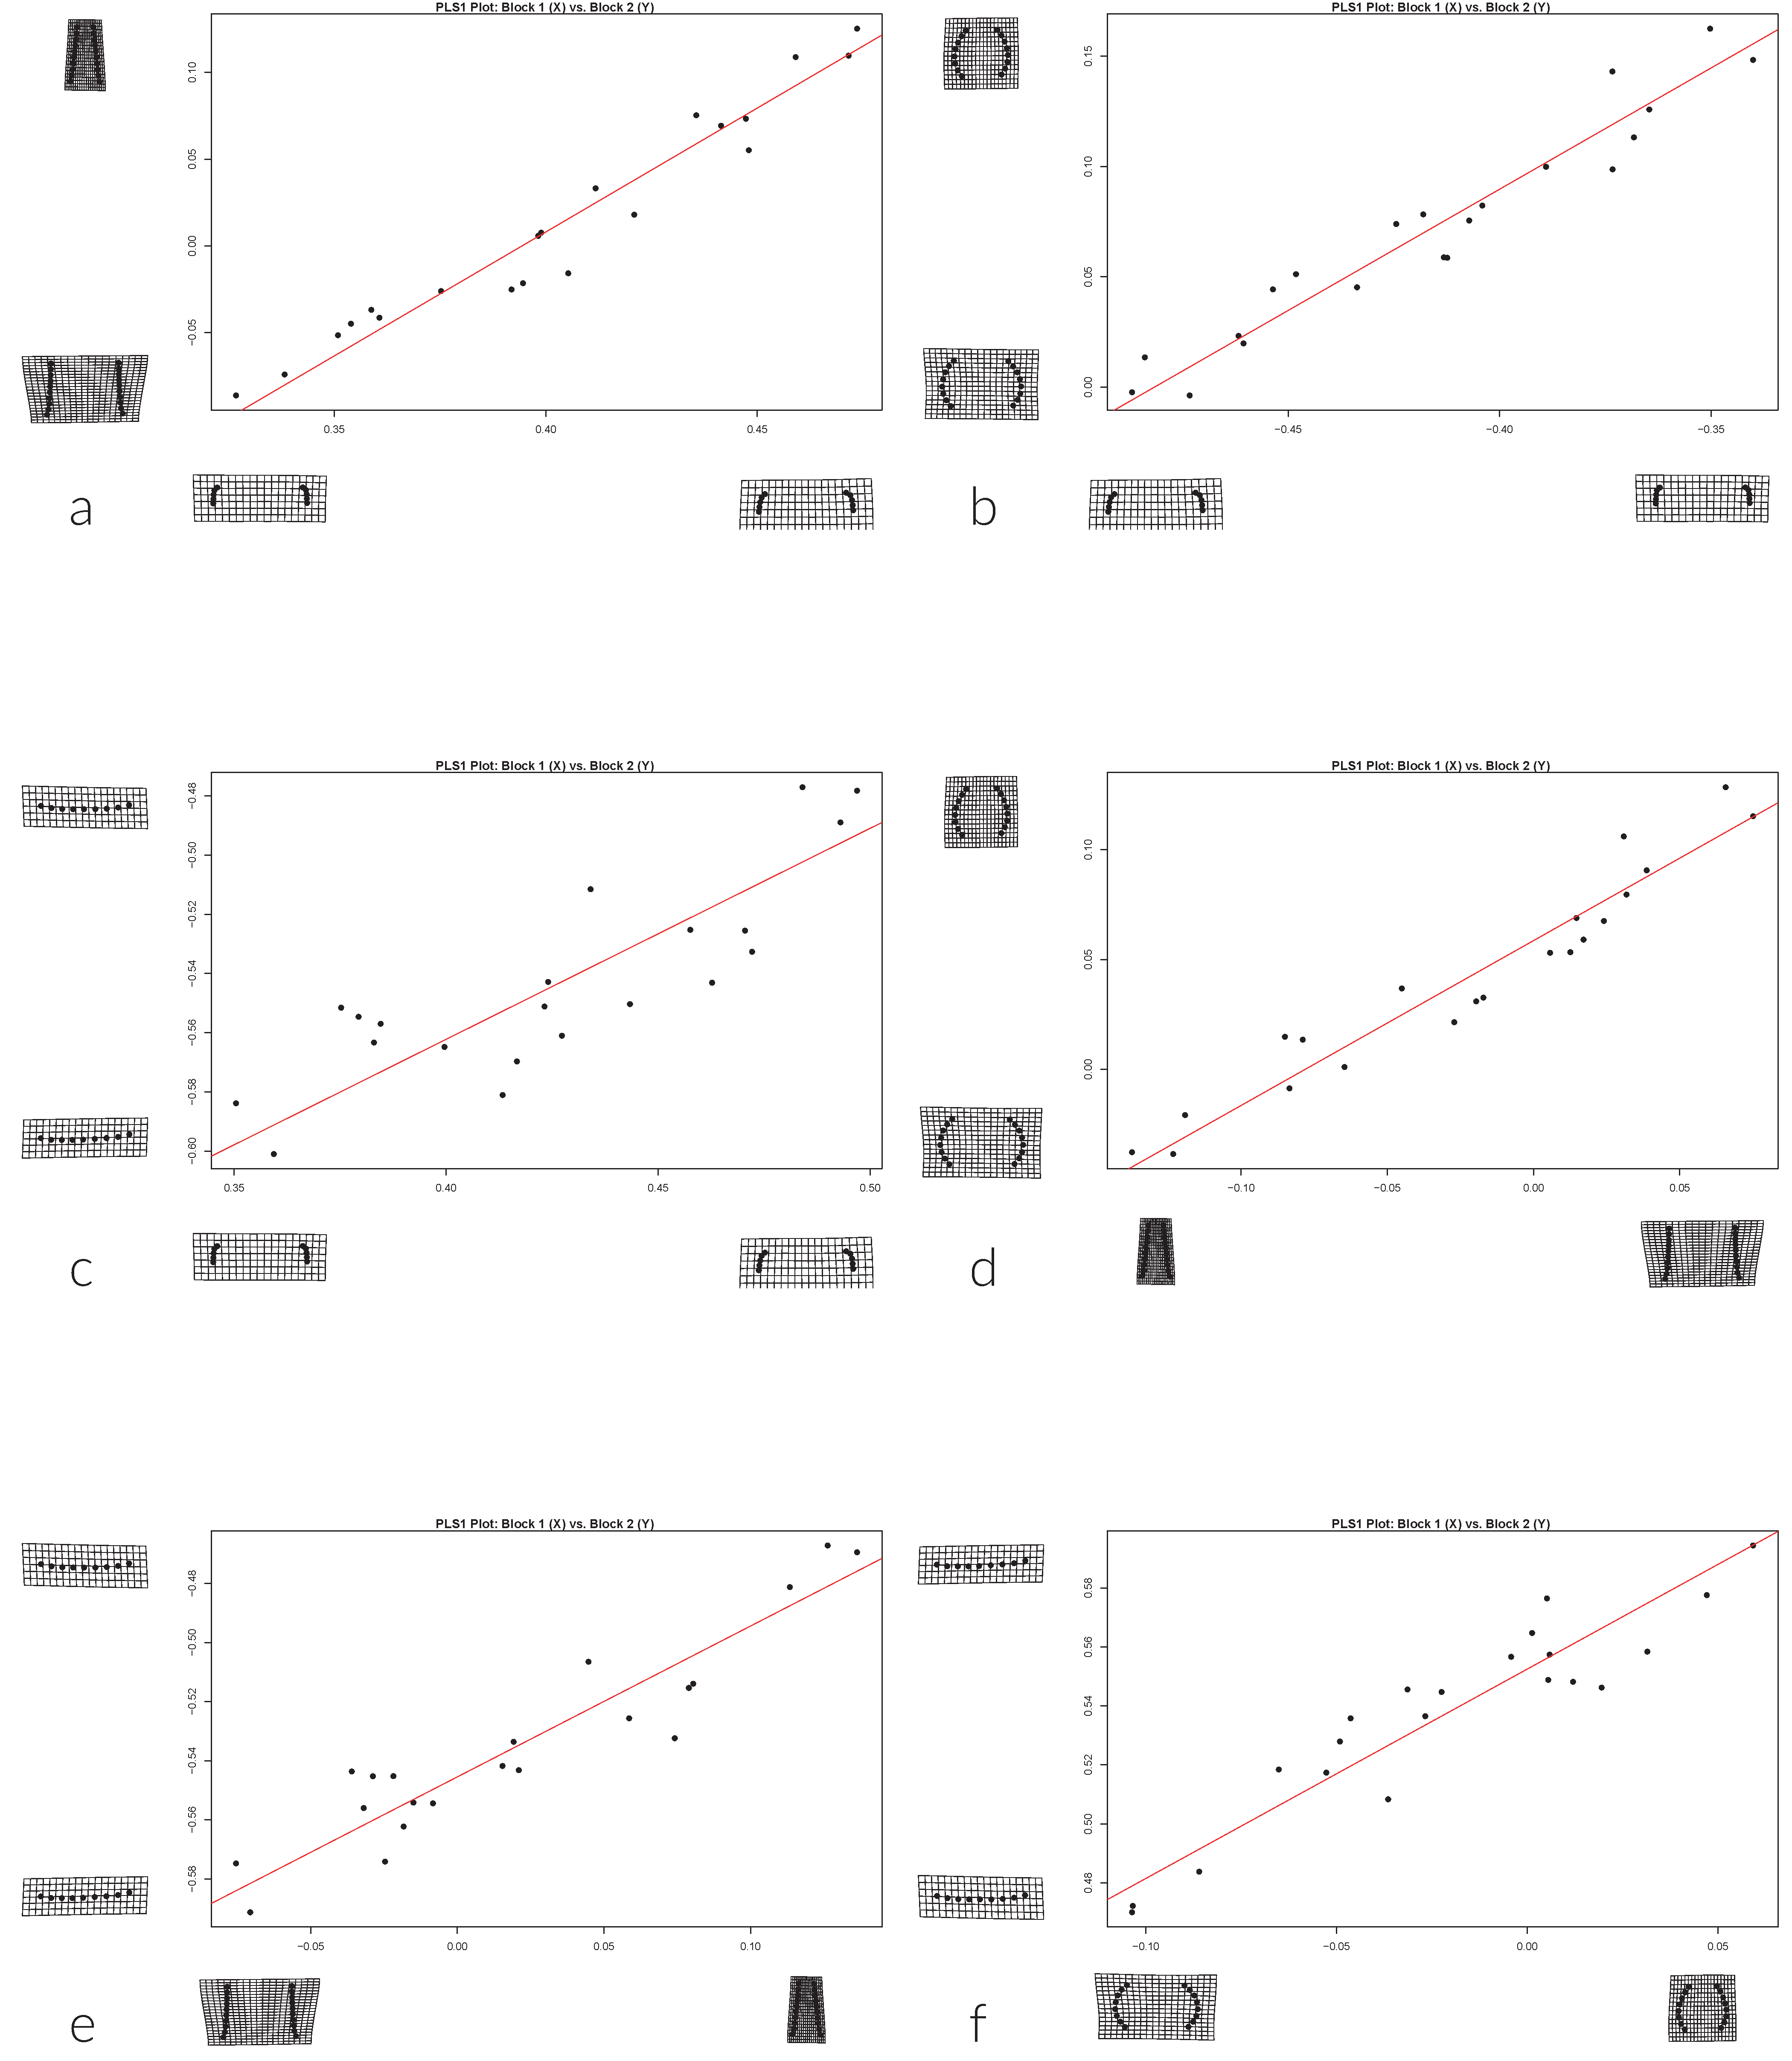
\includegraphics[width=\linewidth]{heintegr}
\caption{Results of 2B-PLS analyses for pairs of morphological components; (a) rim and neck, (b) rim and body, (c) rim and base, (d) neck and body, (e) neck and base, and (f) body and base.}
\label{fig:heintegr}
\end{figure}

\begin{table}[htbp]\centering
\footnotesize
\caption{P-values and effect sizes for morphological integration of trait suites. All results based on 1000 random permutations.}
\centering
\begin{tabular}{lcccccc}
\toprule
 & RIM\textsubscript{neck} & RIM\textsubscript{body} & RIM\textsubscript{base} & NECK\textsubscript{body} & NECK\textsubscript{base} & BODY\textsubscript{base}\\
\midrule
RIM\textsubscript{neck} & 1.0000000 &  &  &  &  & \\
	   & (0.0000000) &  &  &  &  & \\
RIM\textsubscript{body} & 0.2982163 & 1.0000000 &  &  &  & \\
	   & (0.5295376) & (0.0000000) &  &  &  & \\
RIM\textsubscript{base} & 0.1501732 & 0.3012915 & 1.0000000 &  &  & \\
	   & (1.0356908) & (0.52068968) & (0.0000000) &  &  & \\
NECK\textsubscript{body} & 0.2812790 & 0.4820211 & 0.3152516 & 1.0000000 &  & \\
	   & (0.5790463) & (0.04508159) & (0.4810187) & (0.0000000) &  & \\
NECK\textsubscript{base} & 0.3174451 & 0.4836780 & 0.2919756 & 0.4660765 & 1.0000000 & \\
	   & (0.4748551) & (0.04092468) & (0.5476225) & (0.08513646) & (0.0000000) & \\
BODY\textsubscript{base} & 0.1675077 & 0.3321982 & 0.4603731 & 0.3473903 & 0.3215232 & 1.0000000\\
	   & (0.9640607) & (0.43385131) & (0.0994939) & (0.39237570) & (0.46344371) & (0.0000000)\\
\bottomrule
\end{tabular}\\
\smallskip
\textit{Pairwise differences in PLS effect size in parentheses.}\\
\label{tab:Tblmorphinteg}
\end{table}

\subsection{Synthesis of HE bottles with aggregated sample}

The mean consensus configuration and Procrustes residuals were calculated using a GPA for the aggregated sample (Figure ~\ref{fig:gpaagg}). PCA was conducted on scaled, translated, and rotated landmarks, and demonstrate that the first two PCs account for roughly 59 (PC1) and 20.3 (PC2) percent of the variation in bottle shape (Table ~\ref{tab:Tblpca2} and Figure ~\ref{fig:FigPCA2}). Together, PC1 and PC2 account for 79.4 percent of shape variation in the aggregated sample, with each remaining PC representing less than eleven percent of the variation (Table ~\ref{tab:Tblpca2}). The first two PCs are plotted in Figure ~\ref{fig:FigPCA2}, where warp grids represent the shape changes along PC1. This plot indicates that shape changes associated with PC1 articulate most readily with rim, neck, and body shape. Those shape changes associated with PC2 are also dominated by differences in rim, neck, and body shape.

\begin{figure}[ht]\centering
\includegraphics[width=\linewidth]{gpaagg}
\caption{Results of GPA for the aggregated sample. Mean consensus configuration shown in black; samples in gray.}
\label{fig:gpaagg}
\end{figure}

\begin{table}[htbp]\centering
\footnotesize
\caption{Results of PCA for the first 10 PCs (> 99 percent of total variance explained).}
\centering
\begin{tabular}{lp{2cm}p{2cm}p{2cm}}
\toprule
 & SD & PVE & CVE\\
\midrule
PC1 & 0.09246 & 0.59053 & 0.59053\\
PC2 & 0.05433 & 0.20389 & 0.79442\\
PC3 & 0.03994 & 0.11020 & 0.90463\\
PC4 & 0.02350 & 0.03814 & 0.94276\\
PC5 & 0.01773 & 0.02172 & 0.96449\\
PC6 & 0.01305 & 0.01176 & 0.97624\\
PC7 & 0.009666 & 0.006450 & 0.982700\\
PC8 & 0.008099 & 0.004530 & 0.987230\\
PC9 & 0.006923 & 0.003310 & 0.990540\\
PC10 & 0.006142 & 0.002610 & 0.993140\\
\bottomrule
\end{tabular}
\smallskip\\
SD - standard deviation; PVE - percentage variance explained; CVE - cumulative variance explained.
\label{tab:Tblpca2}
\end{table}

\begin{figure}[ht]\centering
\includegraphics[width=\linewidth]{pca-aggwarp.pdf}
\caption{Results of PCA summarising shape variation in the aggregated sample, where red = Hickory Engraved, dark blue = Smithport Plain, green = Keno Trailed, light blue = Taylor Engraved, and black = Belcher Engraved.}
\label{fig:FigPCA2}
\end{figure}

A Procrustes ANOVA was used to test for a significant difference in Caddo bottle shape by size (RRPP = 1000; Rsq = 0.19971; Pr(>F) = 0.001). A second Procrustes ANOVA was used to test for a significant difference in Caddo bottle shape by type (RRPP = 1000; Rsq = 0.41129; Pr(>F) = 0.001), which was followed by a Procrustes ANOVA and pairwise comparison used to identify which types differ significantly in shape, and whether that difference is in magnitude, direction, or both (Table ~\ref{tab:Tbltypex}). 

\begin{table}[htbp]\centering
\footnotesize
\caption{P-values, effect sizes, and least-squares means distance matrix for for advanced Procrustes ANOVA and pairwise test (RRPP = 1000) of shape by type.}
\centering
\begin{tabular}{lrrrrr}
\toprule
 & Belcher Eng & Hickory Eng & Keno Tr & Smithport Pl & Taylor Eng\\
\midrule
Belcher Eng & 1.000 & & & & \\
 & \textit{0.0000000} & & & & \\
  & (0.00000000) & & & & \\
Hickory Eng & \textbf{0.001} & 1.000 & & & \\
 & \textit{4.3918490} & \textit{0.0000000} & & & \\
  & (0.11446991) & (0.00000000) & & & \\
Keno Tr & \textbf{0.031} & \textbf{0.001} & 1.000 & &\\
 & \textit{2.3403817} & \textit{3.974456} & \textit{0.000000} & &\\
  & (0.17142455) & (0.22630873) & (0.0000000) & &\\
Smithport Pl & \textbf{0.001} & \textbf{0.045} & \textbf{0.006} & 1.000 &\\
 & \textit{3.6675308} & \textit{2.017590} & \textit{3.141604} & \textit{0.0000000} &\\
  & (0.21608391) & (0.15298269) & (0.2706105) & (0.0000000) &\\
Taylor Eng & 0.717 & 0.155 & \textbf{0.046} & \textbf{0.041} & 1.000\\
 & \textit{-0.6707131} & \textit{1.039303} & \textit{1.936829} & \textit{1.980969} & \textit{0.0000000}\\
  & (0.04607309) & (0.08509648) & (0.1758952) & (0.1774856) & (0.00000000)\\
\bottomrule
\end{tabular}\\
\smallskip
\textit{Significant differences in bold; effect sizes (z) in italics, LS means distance matrix in parentheses.}
\label{tab:Tbltypex}
\end{table}

A test of morphological disparity indicates that Hickory Engraved and Smithport Plain bottles display a greater range of shape variation among individuals relative to other groups, and differ significantly from the Belcher Engraved and Taylor Engraved bottles (Table ~\ref{tab:TblDISPx}). In a subsequent test, the Formative-Early Caddo bottles (Hickory Engraved and Smithport Plain) were found to encompass a significantly greater range of morphological variability than the Late-Historic Caddo bottles (Belcher Engraved, Keno Trailed, and Taylor Engraved) in the aggregated sample (Table ~\ref{tab:TblDISPx2}). 

\begin{table}[htbp]\centering
\footnotesize
\caption{P-values and pairwise absolute differences between variances for a test of morphological disparity by type (RRPP = 1000).}
\centering
\begin{tabular}{lrrrrr}
\toprule
 & Belcher Eng & Hickory Eng & Keno Tr & Smithport Pl & Taylor Eng\\
\midrule
Belcher Eng & 1.000 & & & &\\
 & (0.0000000000) & & & & \\
Hickory Eng & \textbf{0.002} & 1.000 & & &\\
 & (0.0089995247) & (0.000000000) & & &\\
Keno Tr & 0.900 & 0.072 & 1.000 & &\\
 & (0.0009174212) & (0.009916946) & (0.0000000000) & &\\
Smithport Pl & \textbf{0.021} & 0.495 & 0.087 & 1.000 &\\
 & (0.0134728788) & (0.004473354) & (0.0143903000) & (0.000000000) &\\
Taylor Eng & 0.796 & \textbf{0.049} & 0.732 & 0.070 & 1.000\\
 & (0.0012076110) & (0.007791914) & (0.0021250322) & (0.012265268) & (0.000000000)\\
\bottomrule
\end{tabular}\\
\smallskip
\textit{Significant results in bold; pairwise absolute differences between variances in parentheses.}
\label{tab:TblDISPx}
\end{table}

\begin{table}[htbp]\centering
\footnotesize
\caption{P-values and pairwise absolute differences between variances for a test of morphological disparity by period (RRPP = 1000).}
\centering
\begin{tabular}{lrr}
\toprule
 & Formative-Early & Late-Historic\\
\midrule
Formative-Early & 1.00 &\\
 & (0.000000) &\\
Late-Historic & \textbf{0.016} & 1.00\\
 & (0.007825053) & (0.000000)\\
\bottomrule
\end{tabular}\\
\smallskip
\textit{Significant results in bold; pairwise absolute differences between variances in parentheses.}
\label{tab:TblDISPx2}
\end{table}

\section{Discussion}

Three dimensional meshes were used as the basis for a GM analysis of HE bottle shapes from 10 sites and one collection. This study builds upon results from a previous GM study of the Webb collection, confirms that the posited differences in HE bottle shape identified between the Belcher Mound and Gahagan Mound, Smithport Landing, and Allen Plantation sites are more widespread, highlighting site-specific and (north-south; above/below the confluence of Cypress Bayou and the Red River) geographic variability for the type (Table ~\ref{tab:TblSITE} and Figure ~\ref{fig:compare}). The pairwise test of morphological integration was not significant (Table ~\ref{tab:Tblmorphinteg}), thus the hypothesis that Caddo potters adhered to a template of vessel shape associated with specific decorative motifs must be rejected for this sample. 

\begin{figure}[ht]\centering
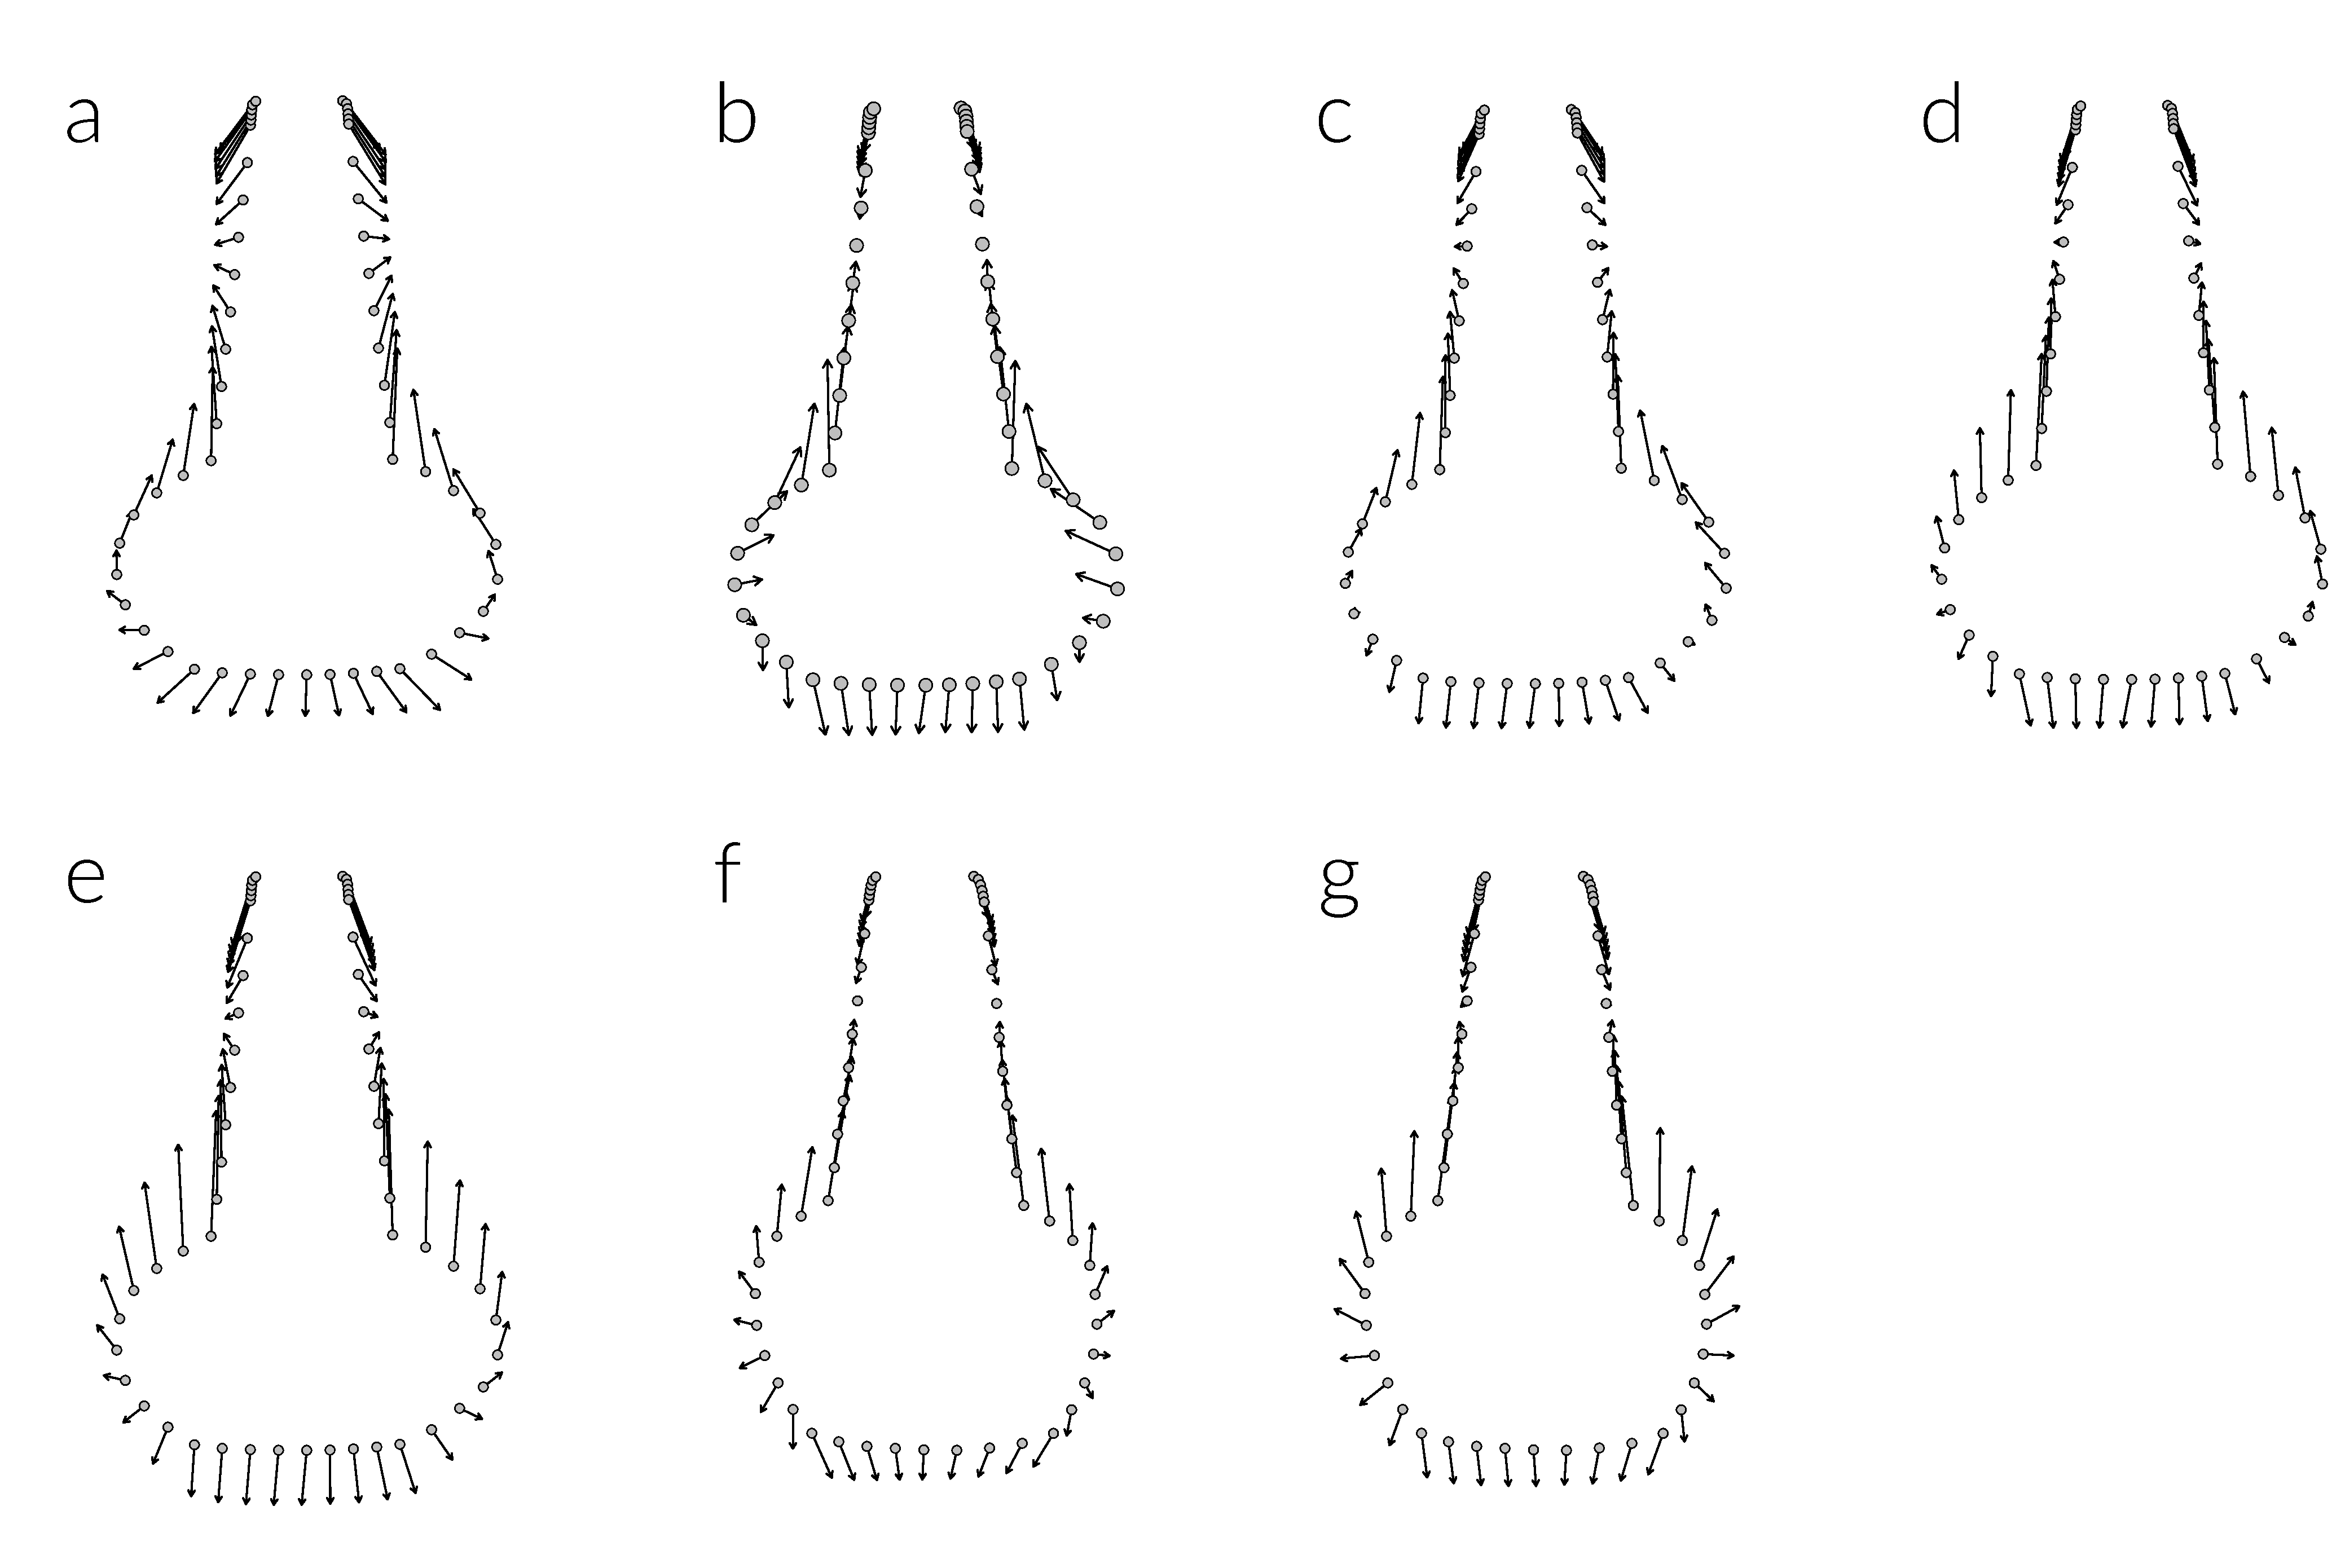
\includegraphics[width=\linewidth]{comparemean}
\caption{Comparison of mean shapes for sites where HE assemblages were found to differ significantly; a, Gahagan Mound (gray) and Belcher Mound; b, Gahagan Mound (gray) and Crenshaw Mound; c, Gahagan Mound (gray) and Haley Place; d, Gahagan Mound (gray) and Paul Mitchell; e, Gahagan Mound (gray) and Pohler Collection; f, Smithport Landing (gray) and Paul Mitchell; and g, Smithport Landing (gray) and Pohler Collection.}
\label{fig:compare}
\end{figure}

Results suggest that the shape of HE bottles may be protean, indicating that variability in Caddo bottle shape was not prescribed, but labile. Spatial differences apparent in HE bottle morphology indicate a possible cultural integument for which the etiology remains unclear. The extent to which this division in bottle shape may be supported by other types and categories of Caddo material culture is unknown; although, results from the previous study of the Webb Collection indicate that Smithport Plain bottle shapes articulate with a similar shift in morphology across the same geographic area. The spatial differences may articulate with differences in HE bottle production; however, the contribution of time remains ill-understood and the putative origin and temporal range for the HE type is not well defined due to a lack of chronometric dates from residues found in HE bottles or contexts from which they were recovered. It is possible that one of the HE bottle shapes represents an earlier manifestation of the type and the other is subsequent; though it is also entirely possible that these two industries were in operation simultaneously.

Efforts to broaden this study through the addition of more samples may aid in further clarifying nuances associated with the variability demonstrated here, which highlight significant differences in the manufacture of HE bottle shape that are dominated largely by geography. The most noticeable differences occur between the bottle bodies and necks of the north-south sample, which generally present as round or pear-shaped in the northern sites and sub-globular in the south, with the juncture of the body and neck evidenced by a more obtuse angle in the north, a (relatively) thinner base of the bottle neck at the neck-body juncture that reduces the amount that HE bottle necks contract toward the rim, and a shorter neck (Figure ~\ref{fig:compare}).

\subsection{Synthesis with the aggregated sample}

In coadunating the HE sample with data from the Webb collection \citep{RN11716}, a broader analysis of Caddo bottle shapes can be considered. The aggregated sample is representative of two periods; one Formative-Early (HE and Smithport Plain), and the other Late-Historic (Belcher Engraved, Keno Trailed, and Taylor Engraved). The advanced Procrustes ANOVA and pairwise test demonstrates some significant differences between the types (Table ~\ref{tab:Tbltypex}). Through the addition of 14 HE bottles, the Formative-Early bottle types in the sample were found to differ significantly in shape, demonstrating the utility of continued iterative improvements to interpretation (Figure ~\ref{fig:comptype}). These results can be contrasted with those from the previous analysis of the Webb collection, where the Formative-Early bottles were not found to differ significantly in shape \citep[Table 5]{RN11716}. Additionally, it was found that a Late-Historic type, Taylor Engraved, does not differ significantly from HE but does differ significantly from Smithport Plain, representing an about-face from the previous analysis \citep[Table 5]{RN11716} (Table ~\ref{tab:Tbltypex} and Figure ~\ref{fig:comptype}).

\begin{figure}[ht]\centering
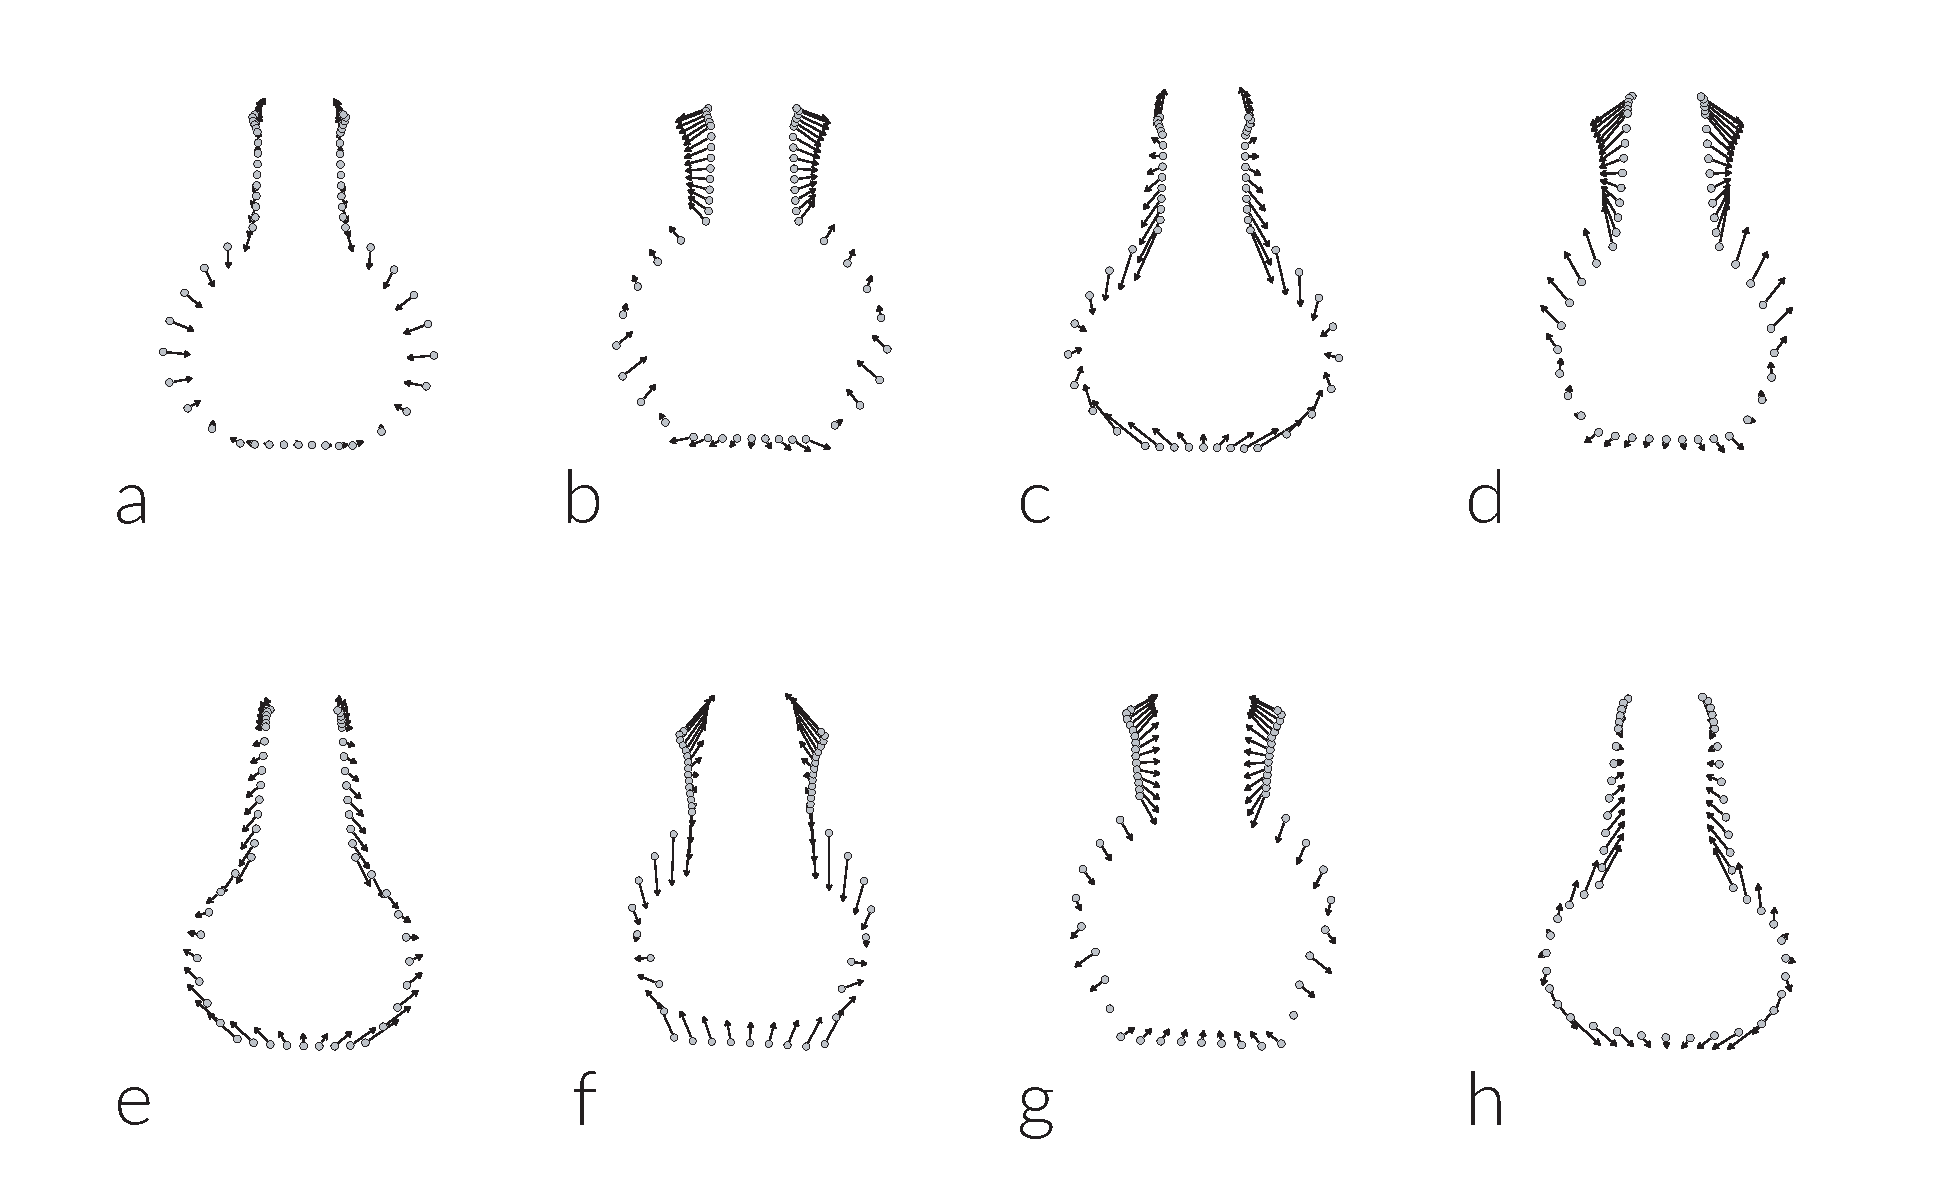
\includegraphics[width=\linewidth]{FigCompType.pdf}
\caption{Comparison of mean bottle shapes by type for those types found to differ significantly (Table ~\ref{tab:Tbltypex}); (a) Belcher Engraved (gray) and Hickory Engraved, (b) Belcher Engraved (gray) and Keno Trailed, (c) Belcher Engraved (gray) and Smithport Plain, (d) Hickory Engraved (gray) and Keno Trailed, (e) Hickory Engraved (gray) and Smithport Plain, (f) Keno Trailed (gray) and Smithport Plain, (g) Keno Trailed (gray) and Taylor Engraved, and (h) Smithport Plain (gray) and Taylor Engraved.}
\label{fig:comptype}
\end{figure}

Results from the test of morphological disparity also differ from the initial analysis; however, to a lesser degree (Table ~\ref{tab:TblDISPx}). In this analysis, the HE bottles occupy a significantly greater range of morphospace than the Taylor Engraved bottles, and the Smithport Plain bottles still occupy a greater range of morphospace than the Belcher Engraved bottles in following with the analysis of the Webb collection, but not the Keno Trailed or Taylor Engraved bottles \citep[Table 6]{RN11716} (Table ~\ref{tab:TblDISPx}). However, the test of morphological disparity by period confirms that the Late-Historic Caddo bottles still occupy a (significantly) more restricted range of morphospace when compared to those from the Formative-Early period.

\subsection{Morphological standardisation}

The morphological attributes employed in this analysis are interpreted to be representative of \textit{intentional attributes} related to morphological characteristics of vessel function \citep{RN250}; the rim, neck, body, and base of Caddo bottles in this instance. The sample of bottles from the Late-Historic period warrants expansion to further test whether---and to what extent---bottle morphology can be said to be restricted. Expansion of the HE sample, and the subsequent analysis of Smithport Plain bottle morphology \citep{RN11801}, extends those findings from the initial study \citep{RN11716}, shifting the interpretation from one of north-south production differences for HE and Smithport Plain bottles to one of differential production for the two types. Additionally, through coadunating the HE bottles with the larger sample, a possible trend toward standardisation is posited that warrants further testing as sample sizes from the differing temporal periods are increased.

Standardisation is relative \citep{RN387,RN13}, is seen as a cultural marker that may have utility in a variety of interpretations, and attempts to measure standardisation have been made using a variety of variables \citep{RN11808}. "Standardization refers to homogeneity in ceramic materials, vessel shape, and/or decoration" \citep[622]{RN28}, while diversity "can be most generally considered as the opposite of standardization" \citep[273]{RN18}. Attributes associated with standardisation may prove dynamic, potentially indicating periods of standardised production as well as periods of creativity and innovation that more readily articulate with diversity \citep{RN7}. In production contexts, standardisation may be seen as the result of minimised labour costs and improvements in efficiency \citep{RN13}. Both standardisation and diversity have utility in characterising tolerance, where a greater range of shapes may be indicative of a higher tolerance, and a lower tolerance by a decrease in variation \citep{RN35}. However, the various functional types and size classes used by prehistoric societies can be a substantive challenge to parse properly from the etic perspective of the archaeologist \citep{RN6008}.

Morphological disparity aided in clarifying a general trend toward standardisation for this sample of Caddo bottles, and morphological integration highlighted those components (i.e., rim, neck, body, and base) and suites of components that covary. The iterative improvement of these results will articulate with the continued development of a dynamic data-driven interpretation of Caddo bottle shapes. Given the absence of direct evidence for ceramic production in the archaeological record of the Caddo, analysts must leverage indirect evidence as a means of generating testable hypotheses. Those hypotheses, if they are to be successful, should not be limited to a single class of artefact, should enlist data for specimens from similar spatial and temporal contexts, and should be supported by analyses at variable scales (Figure ~\ref{fig:profil}).

\begin{figure}[ht]\centering
\includegraphics[width=\linewidth]{figprofil.pdf}
\caption{Scans of incised sherds (left with surface texture applied, and removed at right) collected with a 3D optical profilometer are being used in a study of variable Caddo tool (tip/bit) morphologies used to apply the incisions.}
\label{fig:profil}
\end{figure}

\section{Conclusion}

As sample sizes continue to increase, through the addition of more collections and new discoveries, interpretations should remain dynamic, and demonstrate the many iterative improvements achieved throughout the life cycle of a long-term research design. Systematic comparative studies for aggregated samples of Caddo ceramics are necessary to comprehend the vagaries of vessel morphology. The morphological similarities and differences discussed above have utility in a wide range of research domains, and those bottles used in this analysis can also provide indirect evidence that might be leveraged in studies of Caddo ceramic manufacture and production in the absence of known production areas. A pairwise comparison of morphological integration yielded results that are not significant, thus the hypothesis that Caddo potters adhered to a template of vessel shape associated with specific decorative motifs must be rejected. However, the results of morphological disparity, while differing from those produced in the earlier analysis of the Webb collection, still demonstrate a gradual trend toward standardisation from the Formative-Early to the Late-Historic Caddo periods.

\section*{Acknowledgments}

I extend my gratitude to the Caddo Nation of Oklahoma, the Williamson Museum at Northwestern State University, the Louisiana State Exhibit Museum, the Texas Archeological Research Laboratory, and the LSU Museum of Natural Science for the requisite permissions and access needed to generate the 3D scans of the Caddo bottles. Thanks also to Dean C. Adams, Timothy K. Perttula, Jeffrey R. Girard, Hiram F. (Pete) Gregory, Tad Britt, and Kersten Bergstrom for their constructive criticisms, comments, and suggestions throughout the development of this research design, and to the anonymous reviewers for their comments and constructive criticisms, which further improved this manuscript. Development of this analytical work flow and production of 3D scans from the Clarence H. Webb collection was funded by a grant to the author (P14AP00138) from the National Center for Preservation Technology and Training. Production of 3D scans for repatriated HE bottles from the Crenshaw Mound and the Pohler Collection was funded by a grant to the author by the Caddo Nation of Oklahoma. 

\section*{References}

 \bibliography{mybibfile}

\end{document}